%%%%%%齋藤研究室レジュメテンプレート%%%%%%% 2024

\documentclass[a4j]{jsarticle}
\usepackage[utf8]{inputenc}
\usepackage{amsmath,amssymb,amscd,amsthm}
\usepackage{ascmac,fancybox} 
\usepackage{bm}
\usepackage{mathtools}
\usepackage{multicol}
\usepackage{graphicx}
\usepackage[dvipdfmx]{color}
\usepackage{algorithm}%擬似コードを書く場合
\usepackage{algorithmic}%擬似コードを書く場合
\usepackage{tcolorbox}
\usepackage{marginnote}
%%%% ↓algotithmic の \REQUIRE と \ENSURE の表記を変更する
\renewcommand{\algorithmicrequire}{\textbf{Input:}}
\renewcommand{\algorithmicensure}{\textbf{Output:}}
%%%% ↑algotithmic の \REQUIRE と \ENSURE の表記を変更する
\def \QED{\hfill $\Box$}%証明終了の記号


%%%%%%%本文%%%%%%% 
\title{第7回\\学部3年後期ゼミナール発表資料}
\author{青山和樹}
\date{2024年12月2日}

\begin{document}

\maketitle

%%目的%%
\section*{発表の目的}
テキスト\cite{text}の
\begin{itemize}
	\item 4.1 Markov chains
	\item 4.2 Entropy rate
\end{itemize}
について発表する.


%%目次%%
\tableofcontents

\clearpage

%%本文%%

% チャプター3の漸近等分割性は独立同分布(i.i.d.)なランダムな$X_1, X_2, \ldots , X_n$を記述するのに, 平均して$nH(X)$ビットあれば十分なことを確立した. しかし , ランダムな変数が互いに依存しているならばどうなるだろうか. 特に, ランダム変数が定常過程(stationary process)を形成している場合はどうなるだろう.
% i.i.dの場合と同様に, エントロピー$H(X_1, X_2, \ldots , X_n)$は漸近的に$n$に比例して増加し, その割合を$H(\mathcal{X})$と定義し, エントロピーレートと呼ぶ.

チャプター3の漸近等分割性は独立同分布(i.i.d.)なランダムな$X_1, X_2, \ldots , X_n$を記述するのに, 平均して$nH(X)$ビットあれば十分なことを確立した. ここでは確率変数が互いに依存し, 特に定常過程(stationary process)を形成している場合を考える.


\section{Markov chains}

確率過程(stochastic process)$\{X_i\}$は確率変数の添え字付き列である. 一般に確率変数間には任意の依存関係が存在し得る. またこの過程は, 同時確率関数$\mathbb{P}[(X_1, X_2, \ldots, X_n) = (x_1, x_2, \ldots, x_n)] = p(x_1, x_2, \ldots, x_n), (x_1, x_2, \ldots, x_n) \in \mathcal{X}^n \: \mbox{for} \: n = 1, 2, \ldots$によって, 特徴づけられる.
% \footnote{
% 	\subsection*{式の解釈}
% 	\begin{itemize}
% 		\item $\mathbb{P}$:これは確率を表す記号です. 例えば, 「$\mathbb{P}[A]$」は「事象$A$ が起きる確率」を意味します.
% 		\item $(X_1, X_2, \ldots, X_n)$:これは確率変数の列です. 複数の確率変数$(X_1, X_2, \ldots, X_n)$を一度に扱っています.
% 		\item $(x_1, x_2, \ldots, x_n)$:これは具体的な値の列で, $(X_1, X_2, \ldots, X_n)$がそれぞれ取る値です.
% 		\item $p(x_1, x_2, \ldots, x_n)$:これは確率分布関数(確率質量関数)を表し, 特定の値の組$(x_1, x_2, \ldots, x_n)$を取る確率を表す.
% 		\item $\mathcal{X}^n$:これは確率変数がとりえる値の組の集合を粟田します. 例えば, $\mathcal{X}$が有限集合$\{0, 1\}$ならば, $\mathcal{X}^n$は$(0,0,\ldots, 0)$から$(1,1,\ldots, 1)$のような$n$次元の値の組全体です.
% 	\end{itemize}
% 	\subsection*{文脈の理解}
% 	\begin{itemize}
% 		\item 式の左辺$\mathbb{P}[(X_1, X_2, \ldots, X_n) = (x_1, x_2, \ldots, x_n)]$は, 確率変数$(X_1, X_2, \ldots, X_n)$が特定の値$(x_1, x_2, \ldots, x_n)$を取る確率を表しています.
% 		\item 式の右辺$p(x_1, x_2, \ldots, x_n)$は, この確率を計算するための具体的な確率分布関数です.
% 		\item 「$(x_1, x_2, \ldots, x_n) \in \mathcal{X}^n$」は, 値の取りえる範囲に制約があることを示しています.
% 	\end{itemize}
% }
\\

\begin{itembox}[l]{\textgt{定義 1.1} (定常な確率過程)}
	任意の$n$と任意のシフト$l$, 全ての$x_1, x_2, \ldots, x_n \in X$について
	\begin{align}
		\mathbb{P}[X_1 = x_1, X_2 =x_2, \ldots, X_n = x_n] = \mathbb{P}[X_{l + 1} = x_1, X_{l + 2} =x_2, \ldots, X_{l + n} = x_n]
	\end{align}
	が成り立つとき, 定常であると言う.
	つまり, 確率過程は確率変数列の任意の部分集合の同時分布がそれぞれ時間インデックスのシフトに関して不変であるときである.
\end{itembox}\\

特に, 各確率変数が直前の確率変数にのみ依存し, それ以前の他のすべての確率変数から条件付きで独立している場合, このような過程をマルコフ(Markov)であると言う. \\

\begin{itembox}[l]{\textgt{定義 1.2} (マルコフ連鎖)}
	離散確率過程(discrete stochastic process)$X_1, X_2, \ldots$が全ての$x_1, x_2, \ldots, x_n \in X \: \mbox{for} \: (n =1, 2, \ldots)$について,
	\begin{align}
		\mathbb{P}[X_{n+1} = x_{n+1} | X_n =x_n, X_{n-1} = x_{n-1} \ldots, X_1 = x_1] = \mathbb{P}[X_{n+1} = x_{n+1} | X_n - x_n]
	\end{align}
	が成り立つとき, マルコフ連鎖(Markov cahin)またはマルコフ過程(Markov process)であると言う.
\end{itembox}\\

この場合, 確率変数の同時確率関数は
\begin{align}
	p(x_1, x_2, \ldots, x_n) = p(x_1)p(x_2|x_1)p(x_3|x_2) \dotsm p(x_n|x_{n-1})
\end{align}
と書ける.\\

\begin{itembox}[l]{\textgt{定義 1.3} (時不変なマルコフ連鎖)}
	マルコフ連鎖において, すべての$n = 1, 2, \ldots$について
	\begin{align}
		\mathbb{P}[X_{n+1} = b | X_n = a] = \mathbb{P}[X_2 = b, X_1 = a], \forall a, \forall b \in X
	\end{align}
	が成り立つとき, 時不変であるという.
	つまり, マルコフ連鎖が時間に依存しない場合, すなわち条件付確率$p(x_{n+1}|x_n)$が$n$に依存しない場合である.
\end{itembox}\\

\textgt{注意 1.4} 今後, マルコフ連鎖が特に明記されていない場合, 時不変であると仮定する.
% \footnote{
% 	\subsection*{数学的な簡潔性と解析の容易さ}
% 	\begin{itemize}
% 		\item 時不変の性質\\
% 		      時不変なマルコフ連鎖では, 遷移確率が時間$n$に依存しないため, 計算が大幅に簡単になります. 特に, 遷移確率が一定であるため, 遷移行列$P$を使った解析が可能になります.
% 		\item 予測可能性\\
% 		      時不変な場合, 遷移行列を何度も掛けることで, 将来の状態分布を効率的に計算できます. これにより, 長期的な挙動や定常分布(steady-state distribution)の解析が容易になります.
% 	\end{itemize}
% 	\subsection*{現実のシステムへの適用性}
% 	多くの現実のシステムやプロセスは, ある程度「時間不変」とみなせる場合があります. このようなシステムでは, 時不変な遷移確率を仮定すると, モデル化が簡単になり, 現象の理解や予測がしやすくなります.
% 	\begin{itemize}
% 		\item インフラの状態(電力ネットワーク, 交通ネットワークなど)
% 		\item 顧客行動(特定の時間範囲内での購買行動の傾向)
% 		\item 自然現象(例えば, ある種の天候パターン)
% 	\end{itemize}
% 	\subsection*{一般化されたモデルの基盤としての役割}
% 	\begin{itemize}
% 		\item 特別な場合を含む\\
% 		      時不変なマルコフ連鎖を基本モデルとすることで, さらに複雑な場合(例えば, 時間依存する遷移確率を持つ場合)を拡張として扱いやすくなります.
% 		\item 普遍性\\
% 		      時不変なマルコフ連鎖は, 他の多くの確率過程の基礎となるモデルであり, 確率論や情報理論において広く使用されます.
% 	\end{itemize}
% 	\subsection*{定常分布の解析のため}
% 	時不変なマルコフ連鎖では, 時間が経過すると, 状態分布が「収束」して定常分布(steady-state distribution)になることがあります. この性質は, 多くの応用において重要です.
% 	\begin{itemize}
% 		\item ランダムウォークやページランクアルゴリズム(Googleの検索エンジン)
% 		\item 長期的なシステムの安定性解析
% 		\item 情報理論におけるエントロピー率の計算
% 	\end{itemize}
% }
\\

もし$\{X_i\}$がマルコフ連鎖である場合, $X_n$は時刻$n$における「状態」と呼ばれる. 時不変のマルコフ連鎖は, 初期状態と確率遷移行列(probablility transition matrix)$P = [P_{ij}], i,j \in \{1, 2, \ldots, m\}, \: \mbox{where} \: P_{ij} = \mathbb{P}[X_{n+1} = j | X_n = i]$によって特徴づけられる.\\

\textgt{解説 1.5} マルコフ連鎖において, 任意の状態から他の任意の状態へ有限のステップで正の確率で到達可能な場合, マルコフ連鎖は「既約(irreducible)」であると言う. また, ある状態からその状態自身へ戻る経路の長さの最大公約数が1である場合, そのマルコフ連鎖は非周期的(aperiodic)であると言う.
% \footnote{
% 	\subsection*{既約}
% 	\begin{itemize}
% 		\item 背景
% 		      \begin{itemize}
% 			      \item マルコフ連鎖の解析において, 全ての状態が互いにアクセス可能であることが重要です.
% 			            \item「アクセス可能性」があると, 連鎖が1つの統一されたシステムとして扱えるため, 状態分布が特定のパターン(例えば定常分布)に収束する性質が研究できます.
% 		      \end{itemize}
% 		\item なぜこれが既約性か\\
% 		      「既約(irreducible)」という言葉は数学的には「分割できない」という意味です.
% 		      \begin{itemize}
% 			      \item もし任意の2つの状態間で到達可能でない場合(正の確率で遷移できない場合), そのマルコフ連鎖を2つ以上の「孤立した部分」に分割して考えられます.
% 			      \item 一方で, 任意の状態から他の状態へ正の確率で到達可能である場合, 状態空間全体が1つの「結合した部分」として扱えます.
% 		      \end{itemize}
% 		      この性質により, 既約性を持つマルコフ連鎖は, 全体としての振る舞いを統一的に解析できるようになります.
% 	\end{itemize}
% 	\subsection*{非周期性}
% 	\begin{itemize}
% 		\item 背景
% 		      \begin{itemize}
% 			      \item マルコフ連鎖では, 状態に戻る可能性がある特定のタイミングが周期的にしか現れないと, 連鎖全体がその周期に依存する振る舞いを見せます.
% 			      \item 非周期的である場合, 特定の周期性がなく, 状態に戻るタイミングが任意の時刻に現れる可能性があります.
% 		      \end{itemize}
% 		\item なぜ「最大公約数1」で非周期定期か
% 		      \begin{itemize}
% 			      \item 周期性を説明するために, 「状態$i$に戻るまでの最短ステップ数(経路長)」の集合を考えます. これを$\{t_1,t_2,\ldots\}$とします.
% 			      \item この集合の最大公約数が$d > 1$の場合, 状態$i$に戻れる時刻は$t_1,t_2,\ldots$が常に$d$の倍数になります. このとき, マルコフ連鎖は周期性を持つと言います.
% 			      \item 一方, 最大公約数が1の場合, 任意の自然数$t$に状態$i$に戻る可能性があり, 周期性が存在しないとみなされます.
% 		      \end{itemize}
% 		      例
% 		      \begin{enumerate}
% 			      \item 周期的な場合
% 			            状態$i$に戻れる時刻が常に$t = 2, 4, 6, \ldots$のように偶数であるとします. この場合, 最大公約数は2であり, 周期性2を持ちます.
% 			      \item 非周期的な場合
% 			            状態$i$に戻れる時刻が常に$t = 1, 2, 3, \ldots$のように任意の時刻である場合, 最大公約数は1であり, 周期性がありません.
% 		      \end{enumerate}
% 	\end{itemize}
% 	\subsection*{重要性}
% 	\begin{itemize}
% 		\item 既約性があると, 連鎖全体を1つのシステムとして扱え, 定常分布が存在することが保証されます.
% 		\item 非周期性があると, 定常分布への収束が確実で, 周期的な振る舞いによる偏りがありません.
% 	\end{itemize}
% }
\\

時刻$n$における確率変数の確率関数を$p(x)$とすると, 時刻$n+1$における確率関数は次のように表される.
\footnote{
	\begin{itemize}
		\item 式の意味\\
		      この式は, 次の時刻$n+1$における状態$x_{n+1}$の確率を計算するために, 現在の時刻$n$における全ての状態$x_n$の寄与を足し合わせる, という操作をしています. 式を分解して考えると
		      \begin{enumerate}
			      \item $p(x_n)$:時刻$n$に状態$x_n$にいる確率.
			      \item $P_{x_nx_{n+1}}$:状態$x_n$から$x_{n+1}$に遷移する確率.
			      \item $p(x_n) \cdot P_{x_nx_{n+1}}$:時刻$n+1$に$x_{n+1}$にいるために, 時刻$n$に$x_n$にいる確率関数の貢献.
			      \item $\sum_{x_n}$:すべての$x_n$について足し合わせる.
		      \end{enumerate}
		      時刻$n+1$に$x_{n+1}$にいる確率を求めるためには, 全ての可能な状態$x_n$に対して足し合わせる必要があります.
	\end{itemize}
}
\begin{align}
	p(x_{n+1}) = \sum_{x_n} p(x_n)P_{x_nx_{n+1}}
\end{align}

\textgt{例 1.6} 例えば, さいころの目が$1, 2, 3, 4, 5, 6$の6つの状態を持つとして
\begin{itemize}
	\item $x_n$:時刻$n$に出たサイコロの目.
	\item $x_{n+1}$:時刻$n+1$に出るサイコロの目.
	\item $p(x_n)$:時刻$n$に$x_n$が出る確率.
	\item $P_{x_nx_{n+1}}$:目$x_n$が出た後に目$x_{n+1}$が出るか確率(遷移確率).
\end{itemize}
時刻$n+1$に$x_{n+1}$が出る確率は, 時刻$n$に$x_n$が出て,それが$X_{n+1}$に遷移するすべての可能性を考慮して計算する.\\

\textgt{注意 1.7} 時刻$n+1$における分布が時刻$n$と同じであるような状態の分布を, 定常分布(stationary distribution)と呼ぶ.\\

定常分布と呼ばれる理由は, マルコフ連鎖の初期状態が定常分布に従って選ばれる場合, そのマルコフ連鎖が定常過程を形成するためである. 有限状態のマルコフ連鎖が既約かつ非周期的である場合, 定常分布は一意であり, 任意の初期分布から始めても, 時刻$n$における分布$X_n$は$n \rightarrow \infty$の時, 定常分布に収束する.\\
% \footnote{
% 	\subsection*{定常分布の性質と収束の理由}

% 	有限状態のマルコフ連鎖が既約かつ非周期的である場合, 以下の性質が成り立ちます:

% 	\subsubsection*{1. 定常分布の定義}
% 	定常分布 $\pi = (\pi_1, \pi_2, \ldots, \pi_k)$ とは, 以下を満たす確率分布です:
% 	\begin{align*}
% 		\pi P = \pi
% 	\end{align*}
% 	ここで $P$ はマルコフ連鎖の遷移確率行列を表します. つまり, 状態が定常分布に従って選ばれている場合, 次の時刻でも分布は変化しません.

% 	\subsubsection*{2. 定常分布の一意性}
% 	マルコフ連鎖が既約かつ非周期的であるとき, 以下の理由により定常分布が一意になります:

% 	\begin{itemize}
% 		\item \textbf{既約性:} 任意の状態 $i$ から任意の状態 $j$ に有限のステップで正の確率で到達可能であるため, 状態空間全体が1つの連結したシステムとして扱えます.
% 		\item \textbf{非周期性:} 任意の状態に戻るまでのステップ数が周期性を持たないため, 特定のタイミングに限定されず, 分布が滑らかに混ざり合います.
% 		\item \textbf{ペロン=フロベニウスの定理:} 既約かつ非周期的な確率遷移行列 $P$ は固有値 $1$ に対応する一意の固有ベクトル(定常分布)を持ちます. 他の固有値は絶対値が $1$ 未満であるため, 時間とともに他の成分は消滅します.
% 	\end{itemize}

% 	\subsubsection*{3. 任意の初期分布からの収束}
% 	任意の初期分布 $\mu_0$ に対して, 時刻 $n$ における分布 $\mu_n$ は以下のように遷移します:
% 	\begin{align*}
% 		\mu_{n+1} = \mu_n P.
% 	\end{align*}

% 	このとき, 以下が成り立ちます:
% 	\begin{align*}
% 		\lim_{n \to \infty} \mu_n = \pi,
% 	\end{align*}
% 	ここで $\pi$ は定常分布です.

% 	この収束が成り立つ理由は次の通りです:
% 	\begin{itemize}
% 		\item 既約性により, 状態間の「混ざり合い」が保証されるため, 初期分布の影響が時間とともに薄れていきます.
% 		\item 非周期性により, 状態への到達が特定の周期に縛られず, 任意のタイミングで分布が安定します.
% 		\item 遷移確率行列のべき乗により, 次が成立します:
% 		      \begin{align*}
% 			      \lim_{n \to \infty} P^n = \mathbf{1} \pi,
% 		      \end{align*}
% 		      ここで $\mathbf{1}$ は全ての成分が $1$ の行ベクトルです. このため, 初期分布 $\mu_0$ は時間が経つと定常分布 $\pi$ に収束します.
% 	\end{itemize}

% 	\subsubsection*{4. まとめ}
% 	有限状態のマルコフ連鎖が既約かつ非周期的である場合:
% 	\begin{itemize}
% 		\item 定常分布は一意であり, 存在します.
% 		\item 任意の初期分布から出発しても, 時刻 $n \to \infty$ でその分布は定常分布に収束します.
% 	\end{itemize}
% }

\textgt{例 1.8} 以下に示す遷移確率行列を持つ図\ref{example-1.8}のような2状態マルコフ連鎖を考える.
\begin{align}
	P = \begin{bmatrix}
		    1-\alpha & \alpha  \\
		    \beta    & 1-\beta
	    \end{bmatrix}
\end{align}

定常分布を, それぞれ状態1と状態2の定常確率を成分とするベクトル$\mu$で表すとする. 定常確率は, 方程式$\mu P = \mu$を解くか, より単純に確率のバランスをとることによって求めることができる. 定常分布の場合, 状態遷移グラフのどのカット・セットでも, 純確率流(net probablility flow)はゼロである. これを図\ref{example-1.8}に当てはめると, 次のようになる.
\begin{align}
	\mu_1\alpha = \mu_2\beta
\end{align}
また確率の総和は1であるため
\begin{align}
	\mu_1 = \frac{\beta}{\alpha + \beta},\: \mu_2 = \frac{\alpha}{\alpha + \beta}
\end{align}
もしマルコフ連鎖の初期状態がこの定常分布に従って選ばれる場合, 結果として得られる過程は定常的になる.
% \footnote{
% 	\subsection*{確率のバランスを取るとは?}

% 	「確率のバランスを取る」というのは, \textbf{定常分布}の性質に基づき, 状態遷移グラフにおける\textbf{純確率流がゼロ}になる条件を満たすことを意味します.
% 	これは, 各状態について「その状態に入る確率の総和」と「その状態から出る確率の総和」が等しいことを表します. この条件を満たすと, マルコフ連鎖が時間とともに変化しない分布(定常分布)になります.

% 	\subsection*{数式での表現}

% 	定常分布 $\mu$ は以下の条件を満たします:

% 	\begin{enumerate}
% 		\item \textbf{状態遷移のバランス}
% 		      任意の状態 $i$ について, 状態 $i$ に「入る確率の総和」と「出る確率の総和」が等しいこと:
% 		      \begin{align*}
% 			      \sum_{j} \mu_j P_{ji} = \mu_i
% 		      \end{align*}
% 		      ここで, $\mu_j$ は状態 $j$ の定常確率, $P_{ji}$ は状態 $j$ から状態 $i$ への遷移確率です.

% 		\item \textbf{確率の総和が1}
% 		      定常分布は確率であるため, 全状態の確率の総和は1になります:
% 		      \begin{align*}
% 			      \sum_{i} \mu_i = 1
% 		      \end{align*}
% 	\end{enumerate}

% 	\subsection*{具体例: 2状態マルコフ連鎖}
% 	2つの状態を持つマルコフ連鎖を考えます. 遷移確率行列 $P$ は以下の通りとします:

% 	\begin{align*}
% 		P =
% 		\begin{bmatrix}
% 			1-\alpha & \alpha  \\
% 			\beta    & 1-\beta
% 		\end{bmatrix}
% 	\end{align*}

% 	状態1と状態2の定常確率をそれぞれ $\mu_1, \mu_2$ とすると, 次の条件を満たします:

% 	\begin{align*}
% 		\mu_1 \alpha  & = \mu_2 \beta \\
% 		\mu_1 + \mu_2 & = 1.
% 	\end{align*}

% 	これを解くと, 定常分布は以下のようになります:

% 	\begin{align*}
% 		\mu_1 = \frac{\beta}{\alpha + \beta}, \quad \mu_2 = \frac{\alpha}{\alpha + \beta}.
% 	\end{align*}

% 	\subsection*{定常分布と過程の定常性}
% 	もしマルコフ連鎖の初期状態が定常分布 $\mu$ に従って選ばれる場合, 結果として得られる過程は定常的になります.
% }
% \footnote{

% 	\subsection*{純確率流 (Net Probability Flow)}

% 	\subsubsection*{定義}
% 	純確率流は, あるシステム内で特定の状態 \(i\) における確率の流入と流出の差を表します.
% 	数学的には以下のように定義されます:

% 	\begin{align*}
% 		\text{Net Probability Flow for state } i = \sum_{j} P_{ji} - \sum_{j} P_{ij}
% 	\end{align*}

% 	ここで:
% 	\begin{itemize}
% 		\item \(P_{ji}\): 状態 \(j\) から状態 \(i\) への遷移確率.
% 		\item \(P_{ij}\): 状態 \(i\) から状態 \(j\) への遷移確率.
% 		\item \(\sum_{j} P_{ji}\): 他の状態 \(j\) から状態 \(i\) への流入確率の総和.
% 		\item \(\sum_{j} P_{ij}\): 状態 \(i\) から他の状態 \(j\) への流出確率の総和.
% 	\end{itemize}

% 	\subsubsection*{解釈}
% 	純確率流を用いて, システムが平衡状態にあるか, 非平衡状態にあるかを判別できます.

% 	\begin{enumerate}
% 		\item \textbf{平衡状態}:
% 		      純確率流が0の場合, システムは平衡状態です. この場合, 各状態への確率の流入と流出が完全に釣り合っています.
% 		      \begin{align*}
% 			      \sum_{j} P_{ji} = \sum_{j} P_{ij}, \quad \forall i
% 		      \end{align*}

% 		      例:気体分子がボックス内で均等に分布している状態.

% 		\item \textbf{非平衡状態}:
% 		      純確率流が0でない場合, システムは非平衡状態にあります. この場合, 確率的な変化がまだ進行中です.
% 		      \begin{align*}
% 			      \sum_{j} P_{ji} \neq \sum_{j} P_{ij}, \quad \text{for some } i
% 		      \end{align*}

% 		      例:熱エネルギーが高温から低温へ移動している状況.
% 	\end{enumerate}

% 	\subsubsection*{応用例}
% 	純確率流はさまざまな分野で利用されます:

% 	\begin{itemize}
% 		\item \textbf{マルコフ過程}:
% 		      時間とともに状態が変化する確率的プロセスを解析する際に用いられます.
% 		\item \textbf{統計力学}:
% 		      粒子やエネルギーの分布変化を記述するために使用されます.
% 		\item \textbf{生物学}:
% 		      細胞膜を通じた物質の移動をモデル化する際に利用されます.
% 		\item \textbf{経済学・ネットワーク解析}:
% 		      資金, 情報, または人の流れを解析するためのツールとして使用されます.
% 	\end{itemize}
% }

\textgt{解説 1.9} 時刻$n$における状態$X_n$のエントロピー$H(X_n)$は以下の式で与えられる.
\begin{align}
	H(X_n) = H\left(\frac{\beta}{\alpha + \beta}, \frac{\alpha}{\alpha + \beta}\right)
\end{align}\\

これは過程全体のエントロピー増加率$H(X_1, X_2, \ldots, X_n)$を表すものではない. 確率変数$X$同士の依存関係が影響を与え増加の割合を減らすためである.

\begin{figure}[H]
	\centering
	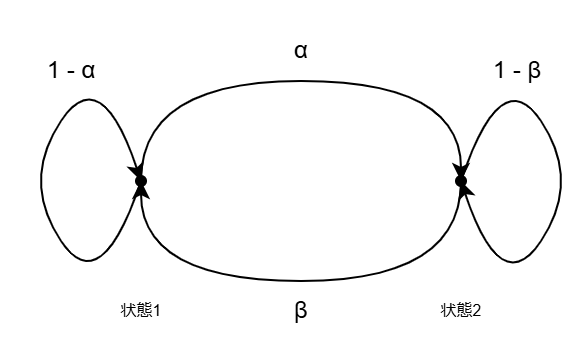
\includegraphics[width = 5.0cm]{example1.8.png}
	\caption{2状態マルコフ連鎖}
	\label{example-1.8}
\end{figure}
% \footnote{
% 	\subsection*{エントロピー $H(X_n)$ と結合エントロピー $H(X_1, X_2, \ldots, X_n)$ の違いについて}

% 	「$H(X_n) = H\left(\frac{\beta}{\alpha + \beta}, \frac{\alpha}{\alpha + \beta}\right)$ は過程全体のエントロピー増加率 $H(X_1, X_2, \ldots, X_n)$ を表さない」という意味について, 以下で詳しく説明します.

% 	\subsubsection*{1. $H(X_n)$ は単一の状態のエントロピー}
% 	エントロピー $H(X_n)$ は, 時刻 $n$ における単一のランダム変数 $X_n$ の不確実性を測るものであり, これは定常分布によって記述されます. マルコフ連鎖が定常分布に従う場合, $H(X_n)$ は以下のように表されます:

% 	\begin{align*}
% 		H(X_n) = -\mu_1 \log \mu_1 - \mu_2 \log \mu_2 = H\left(\frac{\beta}{\alpha + \beta}, \frac{\alpha}{\alpha + \beta}\right)
% 	\end{align*}

% 	ここで, $\mu_1 = \frac{\beta}{\alpha + \beta}$ および $\mu_2 = \frac{\alpha}{\alpha + \beta}$ は定常分布における状態1と状態2の確率を表します.

% 	\subsubsection*{2. $H(X_1, X_2, \ldots, X_n)$ は結合エントロピー}
% 	結合エントロピー $H(X_1, X_2, \ldots, X_n)$ は, $n$ 個のランダム変数をまとめて記述するのに必要な情報量を測るもので, 以下のように定義されます:

% 	\begin{align*}
% 		H(X_1, X_2, \ldots, X_n) = - \sum_{x_1, x_2, \ldots, x_n} \text{Pr}(X_1 = x_1, X_2 = x_2, \ldots, X_n = x_n) \log \text{Pr}(X_1 = x_1, X_2 = x_2, \ldots, X_n = x_n)
% 	\end{align*}

% 	この結合エントロピーは, 単一のエントロピー $H(X_n)$ を単純に足し合わせたものとは異なり, ランダム変数間の依存関係を考慮します.

% 	\subsubsection*{3. 依存関係の影響}
% 	マルコフ連鎖において, ランダム変数 $X_1, X_2, \ldots, X_n$ の間には依存関係があります. この依存関係により, 結合エントロピー $H(X_1, X_2, \ldots, X_n)$ は以下のような不等式を満たします:

% 	\begin{align*}
% 		H(X_1, X_2, \ldots, X_n) \leq \sum_{i=1}^n H(X_i)
% 	\end{align*}

% 	この不等式は, 状態間の依存関係によって情報量の「重複」が発生し, それがエントロピーを減少させることを意味します.

% 	\subsubsection*{4. エントロピー率 $H(X)$}
% 	過程全体のエントロピー増加率は, 結合エントロピー $H(X_1, X_2, \ldots, X_n)$ をランダム変数の数 $n$ で割り, その極限を取ることで定義されます:

% 	\begin{align*}
% 		H(X) = \lim_{n \to \infty} \frac{1}{n} H(X_1, X_2, \ldots, X_n)
% 	\end{align*}

% 	この $H(X)$ は, 1ステップあたりの平均情報量を表し, 過程全体のエントロピー増加率を正確に測る指標となります.

% 	\subsubsection*{5. 結論}
% 	単一のエントロピー $H(X_n)$ は時刻 $n$ における単独の状態の不確実性を表しますが, 結合エントロピー $H(X_1, X_2, \ldots, X_n)$ は, 過程全体の情報量を評価するものであり, 依存関係を考慮した増加率を持ちます. この違いにより, $H(X_n)$ は過程全体のエントロピー増加率を完全には表現しないのです.
% }

\section{Entropy rate}

確率変数の列が$n$個ある場合, その列のエントロピーが$n$に伴ってどのように増加するかを考える.\\

\begin{itembox}[l]{\textgt{定義 2.1} (エントロピーレート)}
	確率過程$\{X_i\}$のエントロピーレート(entropy rate)は次のように定義される.
	\begin{align}
		H(\mathcal{X}) = \lim_{n \rightarrow \infty} \frac{1}{n}H(X_1, X_2, \ldots, X_n)
	\end{align}
	ただし, 極限が存在する時
\end{itembox}\\

\textgt{例 2.2} タイプライター\\

$m$個の等確率の文字を出力する場合を考える. このタイプライターは, 長さ$n$の$m^n$通りの系列を生成でき, それらはすべて等確率である. よって, $H(X_1, X_2, \ldots, X_n) = \log m^n$となり, エントロピーレートは$H(\mathcal{X}) = \log m \: \mbox{(一文字あたりのビット数)}$となる.\\

\textgt{解説 2.3} タイプライターが$m$個の文字を等確率で生成することから, 各文字のエントロピーは
\begin{align}
	H(X) & = - \sum_{i=1}^{m} p(x_i)\log p(x_i)            \\
	     & = - \sum_{i=1}^{m} \frac{1}{m} \log \frac{1}{m} \\
	     & = \log m
\end{align}
独立同分布であるから長さ$n$の文字列全体のエントロピーは
\begin{align}
	H(X_1, X_2, \ldots, X_n) = n \cdot H(X) = n \log m
\end{align}
よって, エントロピーレートは
\begin{align}
	H(\mathcal{X}) = \lim_{n \rightarrow \infty} \frac{1}{n} H(X_1, X_2, \ldots, X_n) = \log m
\end{align}
% \footnote{
% 	\subsection*{エントロピーレートと状態間の遷移}

% 	エントロピーレートが「状態$t$から$t+1$に遷移する際のエントロピー」と解釈されるのは, 文字列が依存関係を持つ場合です.
% 	\begin{itemize}
% 		\item タイプライターの例では, 文字列の各文字が独立しており, 次の文字$X_{t+1}$は前の文字$X_t$に依存しません. この場合, エントロピーレートは単純に一文字あたりの情報量$H(X)$と等しくなります.
% 		      \begin{align*}
% 			      H(\mathcal{X}) = H(X)
% 		      \end{align*}
% 		\item 一方, 文字が依存関係を持つ場合(例えばマルコフ連鎖のような場合), 状態$t$から$t+1$ への遷移に必要な情報量(条件付きエントロピー)を考える必要があります. この場合, エントロピー率は次のように計算されます:
% 		      \begin{align*}
% 			      H(\mathcal{X})= \lim_{n \rightarrow \infty} \frac{1}{n} H(X_1, X_2, \ldots, X_n) = H(X_{n+1} | X_n)
% 		      \end{align*}
% 	\end{itemize}
% }

\textgt{例 2.4} 独立同分布の確率変数\\

$X_1, X_2, \ldots$がi.i.dである場合, 同時エントロピーは
\begin{align}
	H(X_1, X_2, \ldots, X_n) = nH(X)
\end{align}
と表せ, エントロピーレートは
\begin{align}
	H(\mathcal{X}) = \lim \frac{H(X_1, X_2, \ldots, X_n)}{n} = \lim \frac{nH(X_1)}{n} = H(X_1)
\end{align}
と表せる. これは, シンボル当たりのエントロピーレートとして期待させる.\\

\textgt{例 2.5} 独立だが同分布ではない確率変数\\

$X_1, X_2, \ldots$が独立であるが, 同一分布ではない場合, 同時エントロピーは
\begin{align}
	H(X_1, X_2, \ldots, X_n) = \sum_{i=1}^{n} H(X_i)
\end{align}
と表せる.\\

しかし, $H(X_i)$がすべて等しくはなく, $\frac{1}{n} \sum H(X_i)$の極限が存在しないように, $X_1, X_2, \ldots$上の分布の列を選ぶこともできる. 例として, $p_i = \mathbb{P}[X_i = 1]$が定数ではなく$i$の関数であるランダムな2進数列を考え, 極限が存在しないように調整する. 例えば$k = 0, 1, \ldots$として
\begin{align}
	p_i = \begin{cases}
		       & 0.5 \:\:\: 2^k < \log\log i \leq 2^k +1 \mbox{のとき},        \\
		       & 0 \:\:\:\:\:\: 2^k +1 < \log\log i \leq 2^k +2 \mbox{のとき}.
	      \end{cases}
\end{align}
のように定義する.
すると, 指数的に長い$H(X_i)=0$の後に続いて, $H(X_i) = 1$となるような, 任意に長い広がりが生じる. したがって, $H(X_i)$は0と1の間を振動し, 極限を持たない. そのため, この確率過程で$H(\mathcal{X})$は定義されない.\\

\begin{itembox}[l]{\textgt{定義 2.7} (関連するエントロピーレート)}
	\begin{align}
		H^\prime(\mathcal{X}) = \lim_{n \rightarrow \infty} H(X_n | X_{n-1}, X_{n-2}, \ldots X_1)
	\end{align}
	ただし, 極限が存在する時
\end{itembox}\\

\textgt{解説 2.8} 2つの量$H(\mathcal{X}), H^\prime(\mathcal{X})$はエントロピーレートに関する2つの異なる概念に対応する. $H(\mathcal{X})$は$n$個の確率変数に対するシンボル当たりのエントロピーを表し, $H^\prime(\mathcal{X})$は過去が与えられた場合の最後の確率変数に関する条件付エントロピーを表す.\\

\begin{itembox}[l]{\textgt{定理 2.9} (チェザロ平均(cesáro mean))}
	もし$a_n \rightarrow a$かつ$b_n = \frac{1}{n} \sum_{i=1}^{n} a_i$ならば$b_n \rightarrow a$
\end{itembox}\\

\textgt{証明 2.10} 2.9の証明(概要)\\

列$\{a_n\}$のほとんどの項が最終的に$a$に近くなるため, $b_n$(最初の$n$項の平均)は最終的に$a$近づく.\\

\textgt{証明 2.11} 2.9の形式的な証明\\

任意の$\epsilon > 0$として, $a_n \rightarrow a$であるから, ある数$N(\epsilon)$が存在し, すべての$n \geq  N(\epsilon)$に対して\begin{align}
	|a_n - a| \leq \epsilon
\end{align}
を満たす.
したがって,
\begin{align}
	|b_n - a| & = |\frac{1}{n} \sum_{i=1}^{n} (a_i -a)|                                                             \\
	          & \leq \frac{1}{n} \sum_{i=1}^{n} |a_n -a|                                                            \\
	          & = \frac{1}{n} \sum_{i=1}^{N(\epsilon)} |a_n -a| + \frac{1}{n} \sum_{i=N(\epsilon)+1}^{n} |a_n -a|   \\
	          & \leq\frac{1}{n} \sum_{i=1}^{N(\epsilon)} |a_n -a| + \frac{1}{n} \sum_{i=N(\epsilon)+1}^{n} \epsilon \\
	          & = \frac{1}{n} \sum_{i=1}^{N(\epsilon)} |a_n -a| + \frac{n - N(\epsilon)}{n} \epsilon                \\
	          & \leq \frac{1}{n} \sum_{i=1}^{N(\epsilon)} |a_n -a| + \epsilon
\end{align}
がすべての$n \geq  N(\epsilon)$に対して成り立つ. 最初の項は$n \rightarrow \infty$に従って, 0に近づため, $n$を十分大きくとることによって, $|b_n - a| \leq 2\epsilon$とすることができる. よって, $n \rightarrow \infty$に対して$b_n \rightarrow a$となる. \qed\\

\begin{itembox}[l]{\textgt{定理 2.12}}
	定常過程において, 条件付エントロピー$H(X_n | X_{n-1}, X_{n-2}, \ldots, X_1)$は$n$に対して単調非増加であり, 極限$H^\prime(\mathcal{X})$を持つ.
\end{itembox}\\

\textgt{証明 2.13} 条件付エントロピーの定義から条件付けはエントロピーを減らし, 定常性から時間インデックスに関するシフトに対して不変であるから,
\begin{align}
	H(X_{n+1} | X_n, X_{n-1}, \ldots, X_1)
	 & \leq H(X_{n+1} | X_n, X_{n-1}, \ldots, X_2) \\
	 & = H(X_n | X_{n-1}, X_{n-2}, \ldots, X_1)
\end{align}
が成り立つ. よって$H(X_n | X_{n-1}, X_{n-2}, \ldots, X_1)$は非負の減少列であるため, 極限値$H(\mathcal{X})$を持つ.\\

\begin{itembox}[l]{\textgt{定理 2.14}}
	定常過程に対して, 式(10)および式(20)の極限は等しい.
	\begin{align}
		H(\mathcal{X}) = H^\prime(X).
	\end{align}
\end{itembox}\\

\textgt{証明 2.15} チェイン則によって
\begin{align}
	\frac{H(X_1, X_2, \ldots, X_n)}{n} = \frac{1}{n} \sum_{i=1}^{n} H(X_i | X_{i-1}, \ldots, X_1),
\end{align}
つまり, エントロピーレートは条件付きエントロピーの時間平均となる. 条件付きエントロピーが極限値$H^\prime$に収束することから, 定理(2.9)を用いることによって, それら全体にわたる平均は極限値を持ち, それは各項の極限値$H^\prime$に等しい. よって定理(2.12)より
\begin{align}
	H(\mathcal{X}) & = \lim_{n \rightarrow \infty} \frac{1}{n} H(X_1, X_2, \ldots, X_n) = \lim_{n \rightarrow \infty} H(X_n | X_{n-1}, \ldots, X_1) \\
	               & = H^\prime(\mathcal{X})\qed
\end{align}\\

\textgt{解説 2.16} 確率過程のエントロピーレートの重要性は定常エルゴード過程(stationary ergodic process)に対する漸近等分割性に由来する. テキスト\cite{text}16.8にて任意の定常エルゴード過程に対して
\begin{align}
	\frac{1}{n}\log p(X_1, X_2, \ldots, X_n) \rightarrow H(\mathcal{X}) \: (n \rightarrow \infty)
\end{align}
が確率1で成り立つことを証明する. これは第3章の定理を定常エルゴード過程に拡張することを容易にする.\\

第3章でi.i.d.の場合に行ったように, 典型集合を同様の方法で定義でき, 以下が示される.
\begin{itemize}
	\item 典型集合の確率は1に近い
	\item 長さ$n$の典型系列は訳$2^{nH(\mathcal{X})}$個である.
	\item 各典型系列の確率は$2^{-nH(\mathcal{X})}$に近い.
\end{itemize}
したがって, 長さ$n$の典型系列はほぼ$nH(\mathcal{X})$ビットで表現できる. これはエントロピーレートが定常エルゴード過程における平均記述長であることを示している.\\


エントロピーレートはすべての定常過程に対して明確に定義されており, 特に, マルコフ連鎖においてはエントロピーレートの計算が非常に容易である.\\

\textgt{解説 2.17} マルコフ連鎖のエントロピーレート\\

定常マルコフ連鎖におけるエントロピーレートは
\begin{align}
	H(\mathcal{X}) & = H^\prime(\mathcal{X}) = \lim_{n \rightarrow \infty} H(X_n | X_{n-1}, \ldots, X_1) = H(X_n | X_{n-1}) \\
	               & = H(X_2 | X_1)
\end{align}
で与えられる. ここで, 条件付きエントリーは与えられた定常分布によって計算され, 定常分布$\mu$は
\begin{align}
	\mu_j = \sum_{i} \mu_{ij}P_{ij} \:\: \text{(全ての状態jに対して)}
\end{align}
の解として与えられる.\\

\begin{itembox}[l]{\textgt{定理 2.18}}
	$\{X_i\}$を定常分布が$\mu$で確率遷移行列が$P$であるような定常マルコフ連鎖を考える. もし$X_1 \sim \mu$であるなら, エントロピーレートは
	\begin{align}
		H(\mathcal{X}) = - \sum_{i, j} \mu_i P_{ij} \log P_{ij}
	\end{align}
	で表せる
\end{itembox}\\

\textgt{証明 2.19}
\begin{align}
	H(\mathcal{X}) & = H(X_2|X_1)                                                                           \\
	               & = \sum_{i} \mathbb{P}[X_1 = i] \cdot H(X_2 | X_1 = i)                                  \\
	               & =       \sum_{i} \mathbb{P}[X_1 = i] \cdot \left( \sum_{j} -P_{ij} \log P_{ij} \right)
	\\
	               & = \sum_{i} \mu_{i} \left( \sum_{j} -P_{ij} \log P_{ij} \right) \qed
\end{align}\\

\textgt{証明 2.20} 2状態のマルコフ連鎖\\

図\ref{example-1.8}のエントロピーレートは
\begin{align}
	H(\mathcal{X}) = H(X_2|X_1) = \frac{\beta}{\alpha + \beta}H(\alpha) + \frac{\alpha}{\alpha + \beta}H(\beta)
\end{align}
である.\\

\paragraph{備考}

もし, マルコフ連鎖が既約かつ非周期的であるなら,
\begin{enumerate}
	\item 状態上の定常分布は一意である.
	\item 任意の初期分布は$n \rightarrow \infty$で定常分布に収束する.
\end{enumerate}
初期分布が定常分布でなくても, 長期的な挙動に基づくエントロピーレートは式(35)および式(38)に定義されるよう, $H(\mathcal{X})$である.




%%参考文献%%
%\newpage
\begin{thebibliography}{99}
	\bibitem{text}T.M.Cover and J.A.Thomas, Elements of Information Theory, Second Edition, John Wiley \& Sons, 2006.
\end{thebibliography}

\end{document}
